\begin{frame}{three-way TCP handshake}
\begin{tabular}{l@{$\rightarrow$}l|llll}
from & to & flags & seq & ack & data\\
client & server & SYN & $X$ & --- & ---\\
server & client & SYN+ACK & $Y$ & $X+1$ & ---\\
client & server & ACK & $X+1$ & $Y+1$ & ---\\
client & server & ACK & $X+1$ & $Y+1$ & initial data  \\
\end{tabular}
\begin{itemize}
\item $X$, $Y$ selected at random
    \begin{itemize}
    \item random selection to prevent attacker from `spoofing' connection
    \item by sending packets with forged source addresses + guessing what to ACK
    \end{itemize}
\end{itemize}
\end{frame}

\begin{frame}
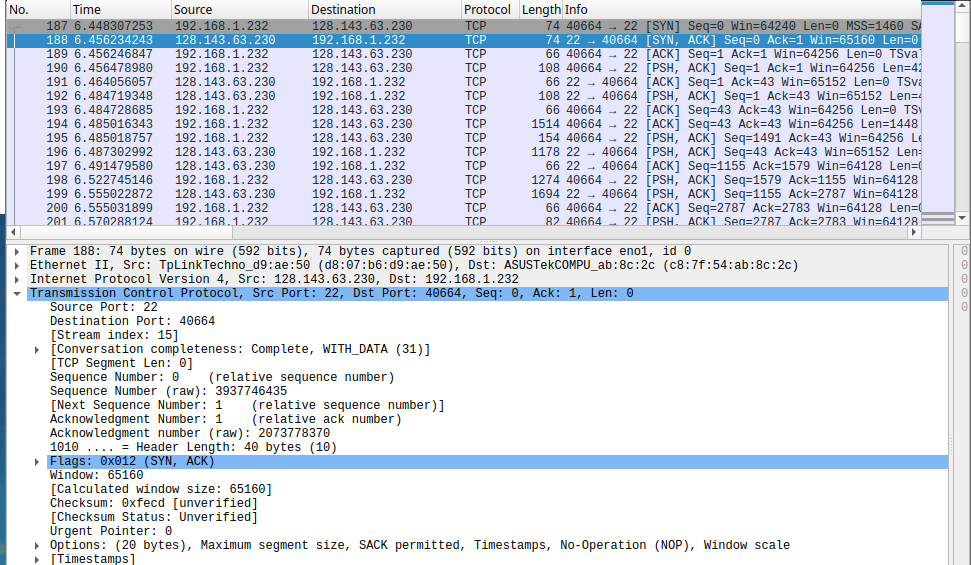
\includegraphics[width=\textwidth]{../sockets/tcp-handshake-wireshark}
\end{frame}

\begin{frame}[fragile]{so many messages?}
    \begin{itemize}
    \item TCP waits full round-trip before sending data; can do better
    \item example: QUIC (figure from RFC 9000, TCP+TLS replacement)
    \end{itemize}
\begin{Verbatim}[fontsize=\fontsize{8}{9}\selectfont]
Client                                                  Server

Initial[0]: CRYPTO[CH]
0-RTT[0]: STREAM[0, "..."] ->

                                 Initial[0]: CRYPTO[SH] ACK[0]
                                  Handshake[0] CRYPTO[EE, FIN]
                          <- 1-RTT[0]: STREAM[1, "..."] ACK[0]

Initial[1]: ACK[0]
Handshake[0]: CRYPTO[FIN], ACK[0]
1-RTT[1]: STREAM[0, "..."] ACK[0] ->

                                          Handshake[1]: ACK[0]
         <- 1-RTT[1]: HANDSHAKE_DONE, STREAM[3, "..."], ACK[1]

Figure 6: Example 0-RTT Handshake
\end{Verbatim}
\end{frame}
